\documentclass[aspectratio=169]{beamer}

% --- THEME ---
\usetheme[progressbar=frametitle]{metropolis}
\useoutertheme{metropolis}
\useinnertheme{metropolis}
\usefonttheme{metropolis}
\usecolortheme{seagull}
\usefonttheme[onlymath]{serif}
% Switch of frame-title colour
\setbeamercolor{palette secondary}{bg=}
\setbeamercolor{frametitle}{parent=palette secondary}

% --- PACKAGES ---
\usepackage[UKenglish]{babel}
\usepackage[utf8]{inputenc}
\usepackage{lmodern}
\usepackage[T1]{fontenc}

% \usepackage{appendixnumberbeamer}
\usepackage{upquote}
% \usetikzlibrary{positioning}
% \usepackage{minted}
% \usepackage{multicol}
\usepackage{xspace}
\usepackage{booktabs}
\usepackage{siunitx}

% --- SETTINGS ---
\graphicspath{{./figures/}}
\setlength{\fboxsep}{0pt}
\frenchspacing
% Avoid font-warning with itemize bullets.
\renewcommand\textbullet{\ensuremath{\bullet}}

% --- OWN COMMANDS ---
\newcommand{\bdra}{\ensuremath{\boldsymbol \Rightarrow }~}
\newcommand{\bdla}{\ensuremath{\boldsymbol \Leftarrow }~}
\newcommand{\dra}{\ensuremath{\Rightarrow }~}
\newcommand{\dla}{\ensuremath{\Leftarrow }~}

\newcommand{\mr}[1]{\mathrm{#1}}

\newcommand{\ohmm}{\ensuremath{\Omega\,}\text{m}\xspace}

\newcommand{\emg}[2]{\texttt{emg#1#2}\xspace}
\newcommand{\empymod}{\texttt{empymod}\xspace}

\newcommand{\rmk}[1]{{\color{red}\bfseries #1}}
\newcommand{\maybe}[1]{{\color{gray} #1}}
\newcommand{\todo}{{\color{red}\texttt{TODO:}}\xspace}
\newcommand{\bm}[1]{{\mathbf{#1}}}

% Add page number to slides
% \definecolor{mygreen}{rgb}{.125,.5,.25}
\definecolor{mygreen}{rgb}{.1,.5,.2}
\definecolor{myblue}{rgb}{0,0,.8}
\newcommand{\ato}{\addtocounter{framenumber}{1}}
\newcommand{\code}[1]{\texttt{\color{mygreen}#1}}

% --- TITLE-STUFF ---
\title{\code{git-intro}}
\subtitle{Introduction to version control, collaborative coding, and continuous integration}
% \date{}
\author{Dieter Werthmüller}
% \institute{}

\hypersetup{colorlinks=true, urlcolor=myblue, citecolor=black, filecolor=black, linkcolor=black}

% --- SLIDES ---
\begin{document}
\metroset{block=fill}  % Fills the block-environment

\ato % ---------------------------------------------------------------------- %
\maketitle

\begin{frame}
  {Outline}
  \tableofcontents
\end{frame}

\ato % ---------------------------------------------------------------------- %
\section{Introduction to \code{git}}

\begin{frame}
  {At the end of the first module you should know\ldots}
  \begin{itemize}\itemsep0.5cm
    \item what \code{git} is and what it is not;
    \item why you should use \code{git};
    \item how to initiate a \code{git} repo;
    \item how to work with \code{git} locally (\code{add}, \code{commit},
      \code{branch}, \code{merge}, \ldots);
    \item how to see changes and to read the log.
  \end{itemize}
\end{frame}

\begin{frame}<5>  % <= <5> : Switch-off overlays
  {Basic rules of code development \& the power of CI}

  \begin{enumerate}
    \item<1-> If you write code, \alert{you are a developer!} (like it or not)
    \item<2-> Code that is not under \alert{version control} does not exist / is
      not reproducible
    \item<3-> Code that is not \alert{properly documented} is not useful
    \item<4-> Code that has no \alert{tests} is broken
  \end{enumerate}
  \vspace{.5cm}

  \uncover<5->{
    \begin{block}
      {Remember:}
    \begin{itemize}
      \item Is it code? \dra Version Control!
      \item Document, document, document, \ldots, and document some more!
      \item Test, test, test, \ldots, and test again! Ideally with benchmarks.
    \end{itemize}
    \end{block}
  }

  \centering

  \uncover<5->{\large \alert{A lot of work \dra Continuous Integration!}}

\end{frame}

\begin{frame}%
  {Version Control: What is it and why should I bother?}

  \begin{description}\itemsep0.2cm
    \item[Why?] \alert{Track your changes and retain entire history};\\
      Reproducibility; Collaboration \& parallel development; Try stuff; \ldots
    \item[What?] Important with \alert{any} (text) file (do not comment out
      large junks!)
    \item[Watch out] \alert{Version Control}\quad \emph{vs}\quad
      \alert{Backup}\quad \emph{vs}\quad \alert{Synchronization}
    \item[Systems]
      \begin{description}
        \item[Centralized] CVS ('86), SVN ('00), \ldots
        \item[Distributed] git ('05, Linus), Mercurial (hg '05), \ldots
        % SVN: Subversions
        % CVS: Concurrent Versions System
      \end{description}
    \item[Hostings]
      \href{https://github.com}{GitHub},
      \href{https://gitlab.com}{GitLab},
      \href{https://bitbucket.org}{Bitbucket},
      \href{https://launchpad.net}{LaunchPad}
  \end{description}

  {\centering \Large \alert{git $\ne$ GitHub/GitLab!}\\}\vfill

\end{frame}

\begin{frame}
  {Useful Links: Git in general}
  \begin{itemize}\itemsep.5em
    \item The Git Book:
      \href{https://git-scm.com/book/en/v2}{git-scm.com/book/en/v2}
    \item Version Control for Scientists:
      \href{https://youtu.be/S4uqsbV-gxY}{youtu.be/S4uqsbV-gxY}
    \item Good, simple primer:
      \href{https://rogerdudler.github.io/git-guide/}%
      {rogerdudler.github.io/git-guide}
    \item GUIs (\code{gitk}): There are GUIs for any OS, just search the web;
      e.g., \href{https://www.hostinger.com/tutorials/best-git-gui-clients/}%
      {hostinger.com/tutorials/best-git-gui-clients}
      {\footnotesize(show GitHub Desk./VS Code/TortoiseGit)}
    \item bash-git-prompt:
      \href{https://github.com/magicmonty/bash-git-prompt}%
      {github.com/magicmonty/bash-git-prompt}
    \item If you screwed up, this might help:
      \href{https://sethrobertson.github.io/GitFixUm/fixup.html}%
      {sethrobertson.github.io/GitFixUm}
    \item Some visualization sites:
      \begin{itemize}
        \item \href{https://dev.to/lydiahallie/cs-visualized-useful-git-commands-37p1}%
      {dev.to/lydiahallie/cs-visualized-useful-git-commands-37p1}
        \item \href{http://onlywei.github.io/explain-git-with-d3}%
            {onlywei.github.io/explain-git-with-d3}
        \item \href{https://marklodato.github.io/visual-git-guide}%
            {marklodato.github.io/visual-git-guide}
      \end{itemize}
  \end{itemize}
\end{frame}

\begin{frame}
  {Licensing}

  \begin{itemize}
    \item Why is it important?
      \begin{itemize}
        \item Putting your code on the web does \emph{NOT} make it open
      \end{itemize}
    \item Copyleft (e.g., GPL) vs permissive (e.g., Apache/MIT/BSD)
    \item Software license $\ne$ creative common licenses (e.g., CC-BY)
    \item \alert{Free as in speech} vs free as in beer vs open-source\\
      (freedom to run, copy, distribute, study, change and improve the software)
    \item How to choose a license?
      \begin{itemize}
        \item \href{https://choosealicense.com}{choosealicense.com}
        \item \href{https://www.gnu.org/licenses/license-recommendations.html}{FSF license list}
        \item Agile Blog: \href{https://agilescientific.com/blog/2021/2/17/which-open-licence-should-i-choose}{Choose a license};
        \href{https://agilescientific.com/blog/2021/5/24/an-open-source-wish-list}{Open-Source wish list}
      \end{itemize}
    \item Free Software Foundation \href{https://www.fsf.org}{fsf.org} (35 years; Linux 29 years)
    \item Electronic Frontier Foundation \href{https://www.eff.org/}{eff.org} (30 years)
    \item Creative Commons \href{https://creativecommons.org}{creativecommons.org} (20 years)
  \end{itemize}

\end{frame}

\begin{frame}
  {Before we get started\ldots\ tell me about you}
    \begin{itemize}\itemsep.5cm
      \item Operating System(s)
      \item Programming Language(s)
      \item Editor(s)
      \item How much knowledge / experience in version control / git / CI
    \end{itemize}

    \vfill
    \centering

    Any other questions before we start?

\end{frame}

\begin{frame}
  {Configuration}
  Check it is installed, and version.
  \begin{itemize}
    \item[\$] \code{git}
    \item[\$] \code{git -{}-version}
  \end{itemize}

  Configuration
  \begin{itemize}
    \item[\$] \code{git config -{}-list}  \# \code{-{}-local} / \code{-{}-global}
    \item[\$] \code{git config -{}-global user.name "Your Name"}
    \item[\$] \code{git config -{}-global user.email "your@email.com"}
    \item[\$] \code{git config -{}-list}
  \end{itemize}

  Location of config file
  \begin{itemize}
    \item \code{$\sim$/.gitconfig} / \code{\$HOME\textbackslash .gitconfig}
    \item \code{local} lives in \code{.git/config};
    there is also a system-wide configuration file
  \end{itemize}
\end{frame}

\begin{frame}
  {First git repository}

  \begin{itemize}
    \item[\$] \code{mkdir testgit}
    \item[\$] \code{cd testgit}
    \item[\$] \code{git status}
    \item[\$] \code{git init}
    \item[\$] \code{git status}
  \end{itemize}

  \vfill

  \dra git is very well documented; use \code{-{}-help} on any command.

\end{frame}

\begin{frame}
  {\code{master} vs \code{main} vs \code{trunk} vs \code{\ldots}}

  git version >= 2.28.0
  \begin{itemize}
    \item[\$] \code{git config -{}-global init.defaultBranch main}
  \end{itemize}
  \vfill

  git version < 2.28.0
  \begin{itemize}
    \item[\$] \code{git init}
    \item[\$] \code{git checkout -b main}  \# Empty repo
    \item[\$] \code{git branch -m main}    \# Non-empty repo
  \end{itemize}
\end{frame}


\begin{frame}
  {Adding and committing -- The git states}

  \begin{columns}
    \column{.5\textwidth}
  \begin{itemize}
    \item[\$] \code{echo “Some text” > myfile.txt}
    \item[\$] \code{git status}
    \item[\$] \code{git add myfile.txt}
    \item[\$] \code{git status}
    \item[\$] \code{git commit -m “First commit”}
    \item[\$] \code{git status}
  \end{itemize}

  \vfill

  Look at
  \begin{itemize}
    \item[\$] \code{git rm -{}-cached myfile.txt}
    \item[\$] \code{git commit -am “Message”}
  \end{itemize}

    \column{.5\textwidth}

  \alert{Three states of git}

    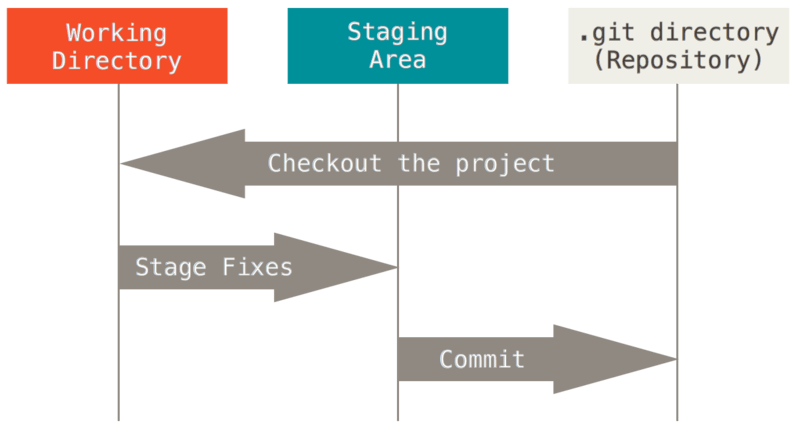
\includegraphics[width=\textwidth]{areas}
  {\tiny Source:
    \href{https://git-scm.com/book/en/v2/Getting-Started-What-is-Git\%3F}%
    {git-scm.com/book/en/v2/Getting-Started-What-is-Git\%3F}}
  \end{columns}

\end{frame}

\begin{frame}
  {What should be in git, what not, ignored files}

  \begin{columns}
    \column{.5\textwidth}

  \begin{itemize}
    \item Yes: Text files
    \item No: Binaries
    \item \emph{Many} exceptions to this
  \end{itemize}

  \vspace{.5cm}

  To ignore files and directories,\\
  there is \code{.gitignore}.

  \vspace{.5cm}

  \dra Look at the \code{.git}-directory!

    \column{.5\textwidth}

  \alert{Stream of snapshots}

    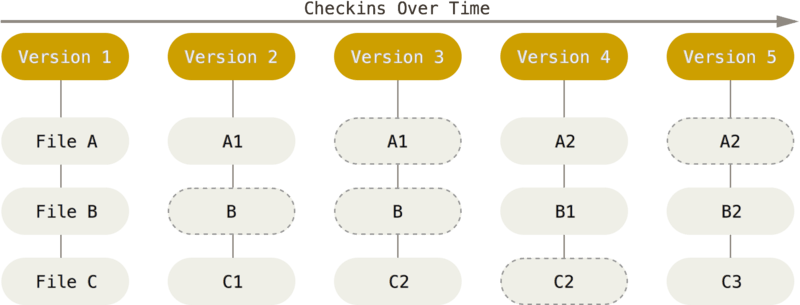
\includegraphics[width=\textwidth]{snapshots}
  {\tiny Source:
    \href{https://git-scm.com/book/en/v2/Getting-Started-What-is-Git\%3F}%
    {git-scm.com/book/en/v2/Getting-Started-What-is-Git\%3F}}
  \end{columns}

\end{frame}

\begin{frame}
  {Exercise I: Getting started}

  \begin{enumerate}\itemsep0.3cm
    \item Create some files.
    \item Make changes to files.
    \item Commit frequently.
    \item Use \code{git status} to observe what happens.
  \end{enumerate}

  \vspace{.5cm}

  Wrap the exercise up by tagging the current version!
  \begin{itemize}
    \item[\$] \code{git tag -a v0.1 -m "Initial version"} \# Annotated tag
    \item[\$] \code{git tag just-to-remember} \# Lightweight tag
  \end{itemize}

\end{frame}


\begin{frame}
  {Branching and merging}

  \begin{columns}
    \column{.5\textwidth}
  Create branches
  \begin{itemize}
    \item[\$] \code{git switch -c featureA}
    \item[\$] \code{git status}
  \end{itemize}

  Switch between branches
  \begin{itemize}
    \item[\$] \code{git switch featureA}
  \end{itemize}

  Merge branche into current one
  \begin{itemize}
    \item[\$] \code{git merge featureA}
  \end{itemize}

  Advanced
  \begin{itemize}
    \item Resolving merge conflicts
    \item Rebasing, squashing, \ldots
  \end{itemize}


    \column{.5\textwidth}

    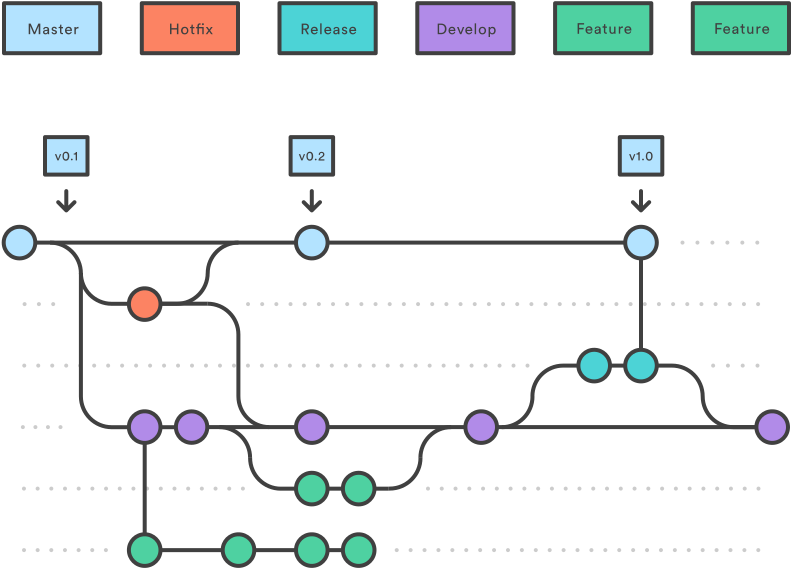
\includegraphics[width=\textwidth]{git-png-branch}
  {\tiny Source: \url{https://www.vippng.com/maxp/hbmmiRx/}}
  \end{columns}

\end{frame}

\begin{frame}
  {Exercise II: Branching and merging}

  \begin{itemize}
    \item Create some branches
    \item Make changes
    \item Merge them back to main
  \end{itemize}

  \vspace{1cm}
  If that is too easy\ldots

  \begin{itemize}
    \item Make some conflicting changes in another branch
    \item Try to resolve the merge conflicts
    \item (We look at it together afterwards)
  \end{itemize}

\end{frame}

\begin{frame}
  {\code{diff} and \code{log}}

  \code{git diff} and \code{git log} can be used to compare branches,
  tags, or hashes in general. In the following a few commands, using
  \code{diff}, but you can also replace it by \code{log}.

  \begin{itemize}
    \item[\$] \code{git diff branch1..branch2}
    \item[\$] \code{git diff tag1..tag2}
    \item[\$] \code{git diff hash1..hash1}
    \item[\$] \code{git diff branch1..branch2 -{}- filename}
  \end{itemize}

\end{frame}


\begin{frame}
  {Graphical log}
  \begin{itemize}
    \item[\$] \code{git log -{}-pretty=oneline}
    \item[\$] \code{git log -{}-graph -{}-pretty}
    \item[\$] \code{git log -{}-graph -{}-oneline -{}-decorate -{}-all}
  \end{itemize}

  Here some commands I copied from
  \href{https://ma.ttias.be/pretty-git-log-in-one-line/}%
  {ma.ttias.be/pretty-git-log-in-one-line}:

  {\small
  \code{git log -{}-graph -{}-pretty=format:'\%Cred\%h\%Creset -\%C(yellow)\%d\%Creset \%s \%Cgreen(\%cr) \%C(bold blue)<\%an>\%Creset' -{}-abbrev-commit}
}

  To not type that every time, you can add a new command \code{logline}:

  {\small
  \code{git config -{}-global alias.logline "log -{}-graph -{}-pretty=format:'\%Cred\%h\%Creset -\%C(yellow)\%d\%Creset \%s \%Cgreen(\%cr) \%C(bold blue)<\%an>\%Creset' -{}-abbrev-commit"}
}

  Then you can run simply \code{git logline}

\end{frame}

\begin{frame}
  {Recap -- Initializing and basic working}
  \begin{block}{Initializing}
  \begin{tabular}{ll}
    \code{git config} & Get and set repository or global options\\
    \code{git init}   & Create an empty Git repository\\
    \code{git status} & Show the working tree status\\
    \code{git <command> -{}-help}   & Help for every git command\\
  \end{tabular}
  \end{block}

  \vfill
  \begin{block}{Adding, committing}
  \begin{tabular}{ll}
    \code{git add}    & Add file contents to the index\\
    \code{git commit} & Record changes to the repository\\
    \code{git commit -{}-amend} & Amend something to previous commit\\
  \end{tabular}
  \end{block}
\end{frame}


\begin{frame}
  {Recap -- File management and history}
  \begin{block}{File management}
  \begin{tabular}{ll}
    \code{git mv}      & Move or rename a files\\
    \code{git rm}      & Remove files\\
    \code{git restore} & Restore working tree files\\
    \code{git restore -{}-staged} & Restore staged files\\
  \end{tabular}
  \end{block}

  \vfill
  \begin{block}{History}
  \begin{tabular}{ll}
    \code{git diff}   & Show changes between commits (see extra slide)\\
    \code{git log}    & Show commit logs (see extra slide)\\
    \code{git grep}   & Print lines matching a pattern\\
  \end{tabular}
  \end{block}

\end{frame}

\begin{frame}
  {Recap -- Branches and advance features}
  \begin{block}{Branches}
  \begin{tabular}{ll}
    \code{git branch}   & List, create, or delete branches\\
    \code{git switch}   & Switch branches (\code{-c} flag to create)\\
    \code{git checkout} & Switch branches or restore files\\
    \code{git merge}    & Join two or more development histories together\\
    \code{git tag}      & Create, list or delete a tag\\
  \end{tabular}
  \end{block}

\end{frame}


\begin{frame}
  {Wrap-up! Now it should be clear\ldots}
  \begin{itemize}\itemsep0.2cm
    \item what \code{git} is and what it is not;
    \item why you should use \code{git};
    \item how to initiate a \code{git} repo;
    \item how to work with \code{git} locally (\code{add}, \code{commit},
      \code{branch}, \code{merge}, \ldots);
    \item how to see changes and to read the log.
  \end{itemize}

  \vfill

  Common question: \alert{How frequently should I commit?}
\end{frame}

\ato % ---------------------------------------------------------------------- %
\section{\code{git} platforms and collaborative coding}

\begin{frame}
  {At the end of the second module you should know\ldots}
  \begin{itemize}\itemsep0.5cm
    \item the difference between \code{git} and \code{git} platforms;
    \item how to suggest a change to any repo on GitHub/GitLab;
    \item how to create a project on GitLab, and use it locally;
    \item how to add an existing repository to GitLab;
    \item how to work and collaborate with others.
  \end{itemize}
\end{frame}

\begin{frame}
  {Collaborative coding}

  We start by looking at GitHub (dominant platform).

  \begin{itemize}
    \item Look at some GitHub repos:
      \begin{itemize}
        \item \href{https://github.com/scipy/scipy}{github.com/scipy/scipy}
        \item \href{https://github.com/simpeg/simpeg}{github.com/simpeg/simpeg}
        \item[\dra] Code; Issues; Pull Requests; \ldots
        \item[\dra] Insights; Releases; Used by; \ldots
        \item[\dra] compare; blame; raw; history; \ldots
        \item[\dra] press the \code{.}
      \end{itemize}
    \item Make an edit on GitHub!
      \href{https://github.com/prisae/learning2git}{github.com/prisae/learning2git}
      \\
      \alert{Make it a habit: learn by giving back to the community!}
  \end{itemize}
\end{frame}

\begin{frame}[t]
  {Vocabulary of different platforms}

  \begin{columns}
    \column{.58\textwidth}
  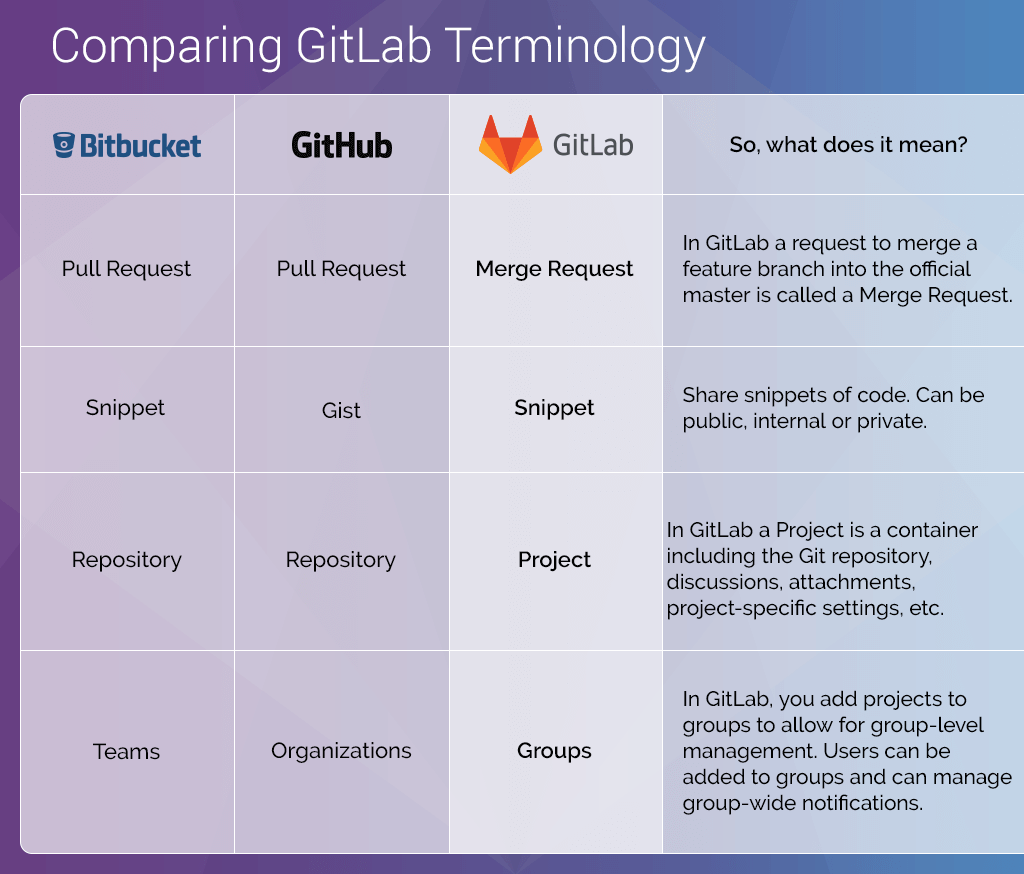
\includegraphics[width=\textwidth]{gitlab-terminology}\\[-.2cm]
  {\tiny Source:
    % \href{https://about.gitlab.com/images/blogimages/gitlab-terminology.png}%
    % {about.gitlab.com/images/blogimages/gitlab-terminology.png}
    \href{https://about.gitlab.com/blog/2016/01/27/comparing-terms-gitlab-github-bitbucket}%
    {about.gitlab.com/blog/2016/01/27/comparing-terms-gitlab-github-bitbucket}
  }

    \column{.4\textwidth}
    \begin{itemize}\itemsep.5cm
      \item Look at GitLab interface
        \begin{itemize}
          \item Personal
          \item Groups
          \item Members
        \end{itemize}
      \item Most important settings/features
    \end{itemize}
  \end{columns}
\end{frame}

\begin{frame}
  {Useful Links: SSH access and documenting}
  \begin{itemize}\itemsep.5cm
    \item Setting up password-free access:
      \begin{itemize}
        \item PASSWORD FREE ACCESS IS CRUCIAL!
        \item \href{https://docs.gitlab.com/ee/user/ssh.html}%
        {docs.gitlab.com/ee/user/ssh.html}
        \item \href{https://docs.github.com/en/github/authenticating-to-github/keeping-your-account-and-data-secure/about-authentication-to-github}%
          {docs.github.com/en/github/authenticating-to-github/keeping-your-account-and-data-secure/about-authentication-to-github}
        \item \href{https://docs.github.com/en/github/authenticating-to-github/connecting-to-github-with-ssh/adding-a-new-ssh-key-to-your-github-account}%
        {docs.github.com/en/github/authenticating-to-github/connecting-to-github-with-ssh/adding-a-new-ssh-key-to-your-github-account}
      \end{itemize}
    \item Markdown:
      \href{https://guides.github.com/features/mastering-markdown}%
      {guides.github.com/features/mastering-markdown}
    \item reStructuredText:
      \href{https://www.writethedocs.org/guide/writing/reStructuredText}%
        {writethedocs.org/guide/writing/reStructuredText}
  \end{itemize}
\end{frame}

\begin{frame}
  {Exercise III: Create a project in your GitLab; collaborate with others}

  \begin{enumerate}\itemsep0.2cm
    \item Go to \href{https://gitlab.tudelft.nl/dieterwerthmul}%
        {gitlab.tudelft.nl/<your-username>}.
    \item Hit \alert{New project} \dra \alert{Create blank project}.
    \item Give it a name and a short description.
    \item Choose visibility and hit \alert{Create project}.
    \item Add some stuff using the Web IDE.
    \item \alert{Search projects of other participants, suggest some changes!}\\
  {\scriptsize \texttt{adaniilidis}; \texttt{amaalfaraj}; \texttt{acuestacano};
  \texttt{andreashadjigeorgiou}; \texttt{akarimzadanzab};
  \texttt{bareveloobando};\\[-.9em] \texttt{dzhang2}; \texttt{edreveloobando};
  \texttt{dverschuur}; \texttt{eslob}; \texttt{jthorbecke};
  \texttt{mikhaildavydenko}; \texttt{sabolhassani}}
    \item Comment/merge/reject/deal with other's suggestions.
    \item At the end, also clone it locally:\\
      \$ \code{git clone git@gitlab.tudelft.nl:<username>/<projectname>}
  \end{enumerate}

\end{frame}

\begin{frame}
  {Exercise IV-a: Add an existing project to GitLab}

  \begin{enumerate}\itemsep0.2cm
    \item Take an existing, local repository.
    \item Create a project on your GitLab as above;\\
      \alert{untick} the \emph{Initialize repository with a README}.
    \item We look together at the \emph{Command line instructions}.
    \item \dra Push your existing git repository following the instructions.
    \item Afterwards:
      \begin{itemize}
        \item Refresh your browser and check your GitLab repo.
        \item Run in your local repository: \code{git remote -v}
      \end{itemize}
  \end{enumerate}

  \begin{itemize}
    \item Note: local repo-folder and remote project folder can have different
      names!
  \end{itemize}

\end{frame}


\begin{frame}
  {Terminology -- repository (local and remote)}
%
  \begin{columns}
    \column{.4\textwidth}
  \begin{itemize}
    \item[\$] \code{git clone}
    \item[\$] \code{git pull}
    \item[\$] \code{git fetch}
    \item[\$] \code{git push}
    \item[\$] \code{git remote -v}
  \end{itemize}

  \vspace{.5cm}

  Advanced
  \begin{itemize}
    \item (soft/hard) fork; upstream
  \end{itemize}
%
    \column{.6\textwidth}
%
    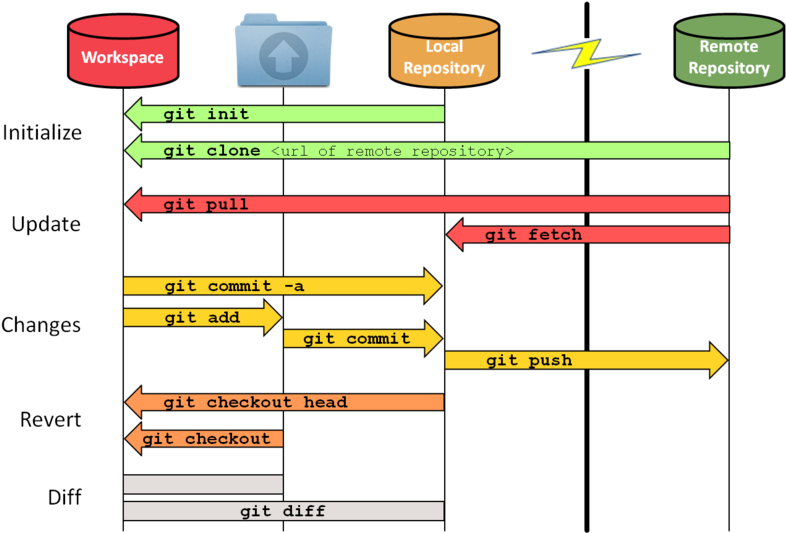
\includegraphics[width=\textwidth]{git-png}
  {\tiny Source: \url{https://www.vippng.com/maxp/hbmmhhh/}}
  \end{columns}
%
\end{frame}

\begin{frame}
  {Exercise IV-b: Working with the local-remote setup}

  \begin{enumerate}\itemsep0.2cm
    \item Local-to-remote
      \begin{itemize}
        \item Make some changes in your local repo.
        \item Commit them and push them to remote.
      \end{itemize}
    \item Remote-to-local
      \begin{itemize}
        \item Make some changes in the web interface.
        \item Fetch the changes to local.
        \item Pull the changes to local.
      \end{itemize}
    \item Pushing/pulling branches and tags.\\
      (\$ \code{git push -{}-set-upstream origin <newbranchname>})\\
      (\$ \code{git push origin -{}-tags})
  \end{enumerate}

\end{frame}


\begin{frame}
  {Exercise V: Collaborating with the Research Group}

  Precursor: Look at branch-setup together.

  \begin{enumerate}\itemsep.5cm
    \item \$ \code{git clone git@gitlab.tudelft.nl:research-group/dummy}
    \item Create a branch (from \code{dev}, \emph{not} from \code{main}).
    \item Make a change.
    \item Commit and push to remote.
    \item Create a merge request to \code{dev} in the web interface.
  \end{enumerate}

\end{frame}

\begin{frame}
  {Recap -- Working with remotes}
  \begin{block}{Remotes}
  \begin{tabular}{ll}
    \code{git clone}  & Clone a repository into a new directory\\
    \code{git push}   & Update remote refs along with associated objects\\
    \code{git fetch}  & Download objects from another repository\\
    \code{git pull}   & Fetch from and integrate with another repository\\
    \code{git remote} & Manage set of tracked repositories\\
  \end{tabular}
  \end{block}

\end{frame}

\begin{frame}
  {Wrap-up! Now it should be clear\ldots}
  \begin{itemize}\itemsep0.2cm
    \item the difference between \code{git} and \code{git} platforms;
    \item how to suggest a change to any repo on GitHub/GitLab;
    \item how to create a project on GitLab, and use it locally;
    \item how to add an existing repository to GitLab;
    \item how to work and collaborate with others.
  \end{itemize}
\end{frame}


\ato % ---------------------------------------------------------------------- %
\section{Reinforcement and advanced topics}

\begin{frame}
  {Today's program}
  \begin{itemize}\itemsep0.5cm
    \item Repeat I: walk-through example, using all commands and learning some
      new
    \item Repeat II: making a collaborative release on
      \href{https://gitlab.tudelft.nl}{gitlab.tudelft.nl}
  \end{itemize}
\end{frame}

\begin{frame}[t]
  {Exercise VI-a: Walk-through -{}-local}
  \tiny
  \vspace{-1.5em}
  config, init, status, log, diff,
  add, commit, restore,
  branch, switch, merge,
  mv, rm,
  tag,
  clone, fetch, pull, push,
  remote\\[2em]


  \begin{columns}[t]
    \column{.33\textwidth}
    (\code{git config})\\[1em]

    Start\\
    \code{mkdir sample}\\
    \code{cd sample}\\
    \code{git init}\\
    \code{git switch -c main}\\
    \code{echo "My Code" > README.md}\\
    \code{git add README.md}\\
    \code{git commit -m "Initial"}\\[1em]

    Branch dev\\
    \code{git switch -c dev}\\
    \code{echo "\# My code" > code.py}\\
    \code{echo "\# My test" > test.py}\\
    \code{git add code.py test.py}\\
    \code{git commit -am "Add code"}\\
    \code{git switch main}\\
    \code{echo "A sample repo" >{}> README.md}\\
    \code{git commit -am "More info"}\\

    \column{.33\textwidth}
    Branch featureA\\
    \code{git switch -c featureA}\\
    \code{echo "New feature" > code2.py}\\
    \code{echo "\# Changelog" > CHANGELOG.md}\\
    \code{echo "- New featureA" >{}> CHANGELOG.md}\\
    \code{git add code2.py CHANGELOG.md}\\
    \code{git commit -am "Feature A"}\\
    \code{git switch main}\\[1em]

    Merge and check\\
    \code{git branch -a}\\
    \code{git merge featureA}\\
    \code{git branch -d featureA}\\
    \code{git status}\\
    \code{git log}\\
    \code{git diff dev..main}\\[1em]

    A change that we regret and undo\\
    \code{echo "bla" >{}> README.md}\\
    \code{git add README.md}\\
    \code{git status}\\
    \code{git restore -{}-staged README.md}\\
    \code{git status}\\
    \code{git restore README.md}\\
    \code{git status}\\[1em]

    \column{.33\textwidth}
    Update dev, keep working\\
    \code{git switch dev}\\
    \code{git merge main}\\
    \code{echo "- Code\&Test" >{}> CHANGELOG.md}\\
    \code{git commit -am "Update log"}\\
    \code{git switch main}\\
    \code{echo "More docs" >{}> README.md}\\
    \code{git commit -am "More docs"}\\
    \code{git merge dev}\\[1em]

    Move and remove\\
    \code{git mv CHANGELOG.md OLD.md}\\
    \code{git commit -am "Rename log"}\\
    \code{git rm OLD.md}\\
    \code{git commit -am "Delete log"}\\
    \code{git status}\\[1em]

    Tag\\
    \code{git tag -a v1.0 -m "Initial Release"}\\[1em]

    Notable ones not used\\
    \code{\# git rebase}\\
    \code{\# git checkout => switch; restore}\\
    we didn't look at \code{.gitignore} here

  \end{columns}

\end{frame}

\begin{frame}[t]
  {Exercise VI-b: Walk-through -{}-remote}
  \tiny
  \vspace{-1.5em}
  config, init, status, log, diff,
  add, commit, restore,
  branch, switch, merge,
  mv, rm,
  tag,
  clone, fetch, pull, push,
  remote\\[2em]

  \begin{columns}[t]
    \column{.6\textwidth}
    On your GitLab or GitHub create an \emph{empty} repo (no README)\\
    \code{git remote add origin git@gitlab.tudelft.nl:dieterwerthmul/sample.git}\\
    \code{git push -u origin -{}-all}\\
    \code{git push -u origin -{}-tags}\\[1em]

    Create a 2nd folder of the same\\
    \code{cd ..}\\
    \code{git clone git@gitlab.tudelft.nl:dieterwerthmul/sample.git twin}\\
    \code{ls}\\[1em]

    Change in «twin»\\
    \code{cd twin}\\
    \code{git remote -v}\\
    \code{echo "Started using remote" >{}> README.md}\\
    \code{git commit -am "Info remote info"}\\
    \code{git status}\\
    \code{git push}\\[1em]

    Update «sample»\\
    \code{cd ../sample}\\
    \code{git fetch}\\
    \code{git status}\\
    \code{git pull}\\
    \code{git status}\\
    \code{cat README.md}\\[1em]

    \column{.4\textwidth}
    Push a new branch\\
    \code{git switch -c new}\\
    \code{echo "Yet another file" > config.cfg}\\
    \code{git add config.cfg}\\
    \code{git commit -am "Add config file"}\\
    \code{git push -{}-set-upstream origin new}\\[1em]

    «add» and «set-upstream» only first time\\
    \code{echo "More config" >{}> config.cfg}\\
    \code{git commit -am "More config"}\\
    \code{git push}\\[2em]

    Comments
    \begin{itemize}
      \item Fetching/pushing new/deleted branches/tags
      \item All these are probably 98\,\% of \code{git}
    \end{itemize}
    If something went awry:
      \begin{itemize}
        \item Internet \& Colleagues
        \item Duplicate \& diff
        \item Clone again \& diff
      \end{itemize}

  \end{columns}

\end{frame}

\begin{frame}
  {Exercise VII: Creating release \code{v2.0} for \code{git2code}}

  We want to create v2.0 of our code. For this, everyone has to add his name to
  the contributor file, and add his file in the source folder. After merging
  all into dev, the owner can merge to main and tag the release.

  \begin{enumerate}
    \item[\$] \code{git clone git@gitlab.tudelft.nl:research-group/git2code}
    \item Checkout \code{dev} (is default branch)
    \item Checkout a branch with your name
    \item Add your name to \code{AUTHORS.md}
    \item Add a file \code{yourname.xyz} with any content in the directory
      \code{src/}
    \item Push it to remote, and create a merge request (to \code{dev}!)
    \item Try to merge each others merge requests into the \code{dev} branch
    \item In the end, we merge it to \code{main} and tag a release
  \end{enumerate}

\end{frame}

\begin{frame}
  {Miscellaneous \code{git}}

  \begin{itemize}
    \item \code{git} is very actively developed:
      \href{https://github.com/git/git/graphs/contributors}%
      {github.com/git/git/graphs/contributors}
    \item \code{git} help online (nice to read):
      \href{https://git-scm.com/docs}{git-scm.com/docs}
    \item[\$] \code{git config -{}-global core.editor vim}\\
      (\code{nano}, \code{vim}, \code{nvim}, \code{emacs}, \code{subl -n -w},
      \code{atom -{}-wait}, \code{code -{}-wait})
  \end{itemize}


  \begin{block}{Not shown}
  \begin{tabular}{ll}
    \code{git fetch upstream} & Keep a forked repo in sync\\
    \code{git cherry-pick}  & Apply a particular commit\\
    \code{git rebase -i}    & Interactive rebasing\\
    \code{git stash}        & Stash dirty working directory away\\
    \code{git bisect}       & To search/find the commit that introduced a bug \\
  \end{tabular}
  \end{block}

\end{frame}

\ato % ---------------------------------------------------------------------- %
\section{Continuous Integration (CI)}

\begin{frame}
  {Today's program}
  \begin{itemize}\itemsep0.5cm
      \item What is it, when is it used
      \item «\emph{Show and tell}» on my codes \empymod \& \emg3d
      \item Make a release of \emg3d
  \end{itemize}
\end{frame}

\begin{frame}
  {Continuous Integration (CI) -- What/Why}

  \begin{block}{In its original sense}
    The practices of collaborating and \emph{merging frequently} to a shared
    version of the code (see
    \href{https://en.wikipedia.org/wiki/Continuous_integration}%
    {en.wikipedia.org/wiki/Continuous\_integration}).
  \end{block}

  \begin{itemize}
    \item This is a lot of work.
    \item Automate the test-review-QC-build-deploy workflow as much as possible.
    \item Goes well with \emph{Version control};
      \href{https://en.wikipedia.org/wiki/Test-driven_development}%
      {Test-driven development};
      \href{https://en.wikipedia.org/wiki/Release_early,_release_often}%
      {Release early, release often} philosophy; and other ideas.
  \end{itemize}

\end{frame}

\begin{frame}
  {Continuous Integration (CI) -- Advantages}

  \begin{itemize}
    \item No last minute chaos on «integration day»!
    \item Helps to produce more modular code (refactor; less complexity).
    \item Reduces maintainer load when accepting contributions.
    \item Much more likely to refactor.
  \end{itemize}

  \center
  \alert{It is very easy to write complex code. It is hard to write simple
  code.}

\end{frame}

\begin{frame}
  {CI \& Automation on the example of \texttt{empymod}}

  \begin{itemize}
    \item Commit to GitHub
    \item GitHub Actions - run all tests
      \begin{itemize}
        \item Linux, MacOS, Windows
        \item Different Python versions
        \item Report to coveralls (code coverage)
        \item Check all hyperlinks
        \item Deploy to PyPi and conda-forge (\emph{if tag})
      \end{itemize}
    \item Codacy (code quality)
    \item ReadTheDocs and Gallery
    \item Mint DOI at Zenodo (\emph{if tag})
    \item Benchmarks (\texttt{asv}, \emph{manual})
  \end{itemize}

  \vfill

  \alert{All of them are \emph{free} (for open-source projects)}

\end{frame}

\begin{frame}
  {CI: Fast/automatic deployment}

  \alert{We create a release of emg3d.}

\end{frame}

\end{document}
